\documentclass[12 pt]{scrartcl}
\usepackage{setspace}
\onehalfspacing
\usepackage{amsmath,amssymb,amsfonts,amsthm,mathtools}
\usepackage[english]{babel}
\usepackage[T1]{fontenc}
\usepackage[utf8x]{inputenc}
\usepackage{lmodern}
\usepackage{dsfont}
\usepackage{bbm}
\usepackage[round]{natbib}
\usepackage{color} 
\usepackage[defaultlines=2,all]{nowidow}
\usepackage{caption}
\usepackage[labelformat=simple]{subcaption}
\usepackage{graphicx}
\renewcommand\thesubfigure{(\alph{subfigure})}

\setlength\parindent{0pt}
\setlength{\parskip}{6pt plus 1pt minus 1pt}

\newcommand{\red}{\textcolor{red}}


\begin{document}



\begin{titlepage}
	\centering
	{\scshape\LARGE TU Dortmund \par}
	\vspace{1cm}
	{\scshape\Large Introductory Case Studies \par}
	\vspace{2cm}
	{\huge\bfseries Project {1}: {Descriptive analysis of demographic data}\par}
	\vspace{2cm}
	{\Large Lecturers:\\
		Prof.\ Dr.\ Katja Ickstadt\\
		M.\ Sc.\ Zeyu Ding\\
		M.\ Sc.\ Yassine Talleb \par}
	\vspace{1cm}
	{\Large Author: {Ojekunle Taiwo} \par}
	\vspace{0.5 cm}
	{\Large Group number: {10}\par}
	\vspace{0.5 cm}
	{\Large Group members: {Opeyemi Ayanwale, Azeezat Mosunmade Mustapha, Divya Prima Crasta, Taiwo Ojekunle}}
	\vfill
	{\large \today\par}
\end{titlepage}



\tableofcontents
\thispagestyle{empty}

\cleardoublepage

\setcounter{page}{1}

\section{Introduction}

This report presents a descriptive analysis of the demographic data extracted from the International Data Base(IDB) on all states and regions that are recognized by the US Department of State. The data set contains census data from the years 2002 - 2022 which includes life expectancy at birth and under age 5 mortality rates for 227 countries in different regions. Descriptive analysis is a type of analysis that explains or analyzes a data set with the help of statistical visualization methods such as histograms, boxplots, and scatterplots to learn more about the variables in the population. The importance of this analysis is to enable us to understand more about the population by observing the characteristics of the population such as the life expectancy and mortality rate in our dataset which are important variables in accessing the quality of the health sector. Another importance of descriptive analysis for demographic data is to observe trends and make better decisions regarding the population.

The purpose of this report is to describe the frequency distribution of variables in our data set to get a better understanding of the relationship between variables and check for bivariate correlations between variables, also want to check for variability within individual subregions and between different subregions and trends of variables over the last 20 years. Statistical methods such as the measures of central tendency (mean and median), measures of dispersion(Quantiles, Interquartile range, variance, and standard deviation), and visualization (histogram, boxplot, scatterplot) would be used to analyze our dataset to actualize our purpose for this report.

In the second section, we will look more into our data, get an overview of our dataset and assess the quality of the data before we perform any descriptive analysis which will be written in detail in section three, where we expatiate on the methods we would use in our analysis. The third section explains a lot about explanatory data analysis with its definitions, properties, assumptions, and its interpretations. In section four, these statistical methods are applied to our given dataset and the results are interpreted. And finally, in section 5, we give the summary of the observations gotten from applying the methods explained in section four.



\section{Problem statement}


\subsection{Data Set and Data Quality}

The data set used in this project is extracted from the International Data Base (IDB) and was compiled by the US Department of State with information from state institutions such as censuses, surveys, or administrative records. The data set contains 454 countries with ten(10) columns for country names, subregions, regions, years, life expectancy at birth for both sexes(LEB), life expectancy at birth for males(LEM), life expectancy at birth for females(LEF), under age 5 mortality for both sexes(MB), under age 5 mortality for males(MM) and under age 5 mortality for females(MF). There are five (5) unique regions: Asia, Africa, Americas, Europe, and Oceania with twenty-one (21) sub-regions that classify the countries.

Life expectancy at birth is defined as the maximum possible number of years a group of people under the same constant variables such as year of birth and mortality are expected to live. Under-age 5 mortality is defined as the number of deaths of children under 5 years of age from a cohort of 1000 live births.  The data quality is fairly okay because it contains forty-four (44)  missing values in total. Life expectancy at birth for both sexes, life expectancy at birth for males, life expectancy at birth for females, under age 5 mortality for both sexes, under age 5 mortality for males,  and under age 5 mortality for females all contain six (6) missing values and also four (4) missing values in regions and subregion columns for 2022. Nevertheless, the mean was used as a method for imputing the missing values in increasing the quality of our data set in the numerical columns. For regions and sub-regions columns, missing values are replaced with the actual region and sub-region names.



\subsection{Project objectives}
In this project, the aim of this descriptive analysis is to describe the frequency distributions of the variables while also considering the differences between the sexes and regions. Here we use statistical visualization such as histograms to get an overview of the data and also help in getting the measures of central tendency (mean and median) and dispersion (standard deviation and variance) which help describes the distribution of mortality and life expectancy rates for the year 2022 with the difference between the sexes and region. Secondly, we aim to check for the variability of values if they are comparatively homogenous within subregions and heterogenous between different subregions and the variability can also be checked with the help of visualizing our data with boxplots comparing the range and interquartile range of the boxplots to check for variability in our data set for the year 2022.
Thirdly, we would like to check if there are bivariate relationships between the variables and this can be checked with the help of plotting a scatter plot for our data and obtaining the correlation coefficient to quantify the strength of the relationship between variables for the year 2022.
Finally, we want to compare how the values of the variables changed over the last 20 years comparing the year 2002 with 2022 which can be done with the help of constructing a boxplot for variables in 2002 and 2022.



\section{Statistical Methods}

In this section, we would discuss the statistical methods that would be applied in the analyses of our dataset with respect to the objectives of the project. R software (R version 4.3.0 (2023-04-21)) was used for the visualization to provide the solution to the task given with the help of packages like ggplot.

\subsection{Measures of Central Tendency}

Measures of Central Tendency

A measure of central tendency is a statistical measure that describes a whole data set with a value that represents the middle or the center of the distribution. We would be discussing two measures of central tendency in this project which are mean and median. \citep{Hay}.
\subsubsection{Mean}

Amongst the different types of mean which include arithmetic mean, geometric mean, and harmonic mean. In this report, we will be using the arithmetic mean for our analysis, and it can be defined as the sum of numbers divided by the total count of numbers. In order words, the mean of a distribution of observations  $x_1, x_2, \ldots, x_n$ is defined as $\bar{x} = \frac{1}{n}\sum_{i=1}^{n} x_i$, $\text{for }i=1,\ldots, n$. Where $\bar{x}$ represents the sample mean and $x_i$ represents observations in a distribution.

The arithmetic mean is sensitive to outliers or extreme values and it is most suitable for homogenous data sets. (Christopher Hay - Jahans,2018, p.73 - 74).


\subsubsection{Median}
 
 If a sample of $x_1, x_2, \ldots, x_n$ is arranged in ascending order , the median $x_bar$ is defined as
 
  $\tilde{x} = \begin{cases}x_{(n+1)/2} & \text{if $n$ is odd} \\\frac{x_{n/2}+x_{(n/2)+1}}{2} & \text{if $n$ is even} \end{cases}$ 
 
 where $\tilde{x}$ is the median of the distribution.
 
The median is not sensitive to extreme values and outliers in a sample and it is the most preferred measure of central tendency when dealing with data that contains extreme values. 
In general, the mean is preferred for a data set with no outliers while the Median is preferred for data sets with outliers for the measure of central tendency. (Christopher Hay - Jahans,2018, p.75 - 76).
 
 
\subsection{Measure of dispersion}

The measure of dispersion can be defined as the extent to which a distribution is stretched or squeezed. Variance, standard deviation, range, and interquartile range are some examples of dispersion that would be used in our analysis. (Jiawei Han and Micheline Kamber, 2nd edition, p.53 - 54).

\subsubsection{Variance and Standard Deviation}

In the measure of how a set of observations $x_1, x_2, \ldots, x_n$ in a data varies from the mean value of the data set, variance is a useful tool in calculating the spread and it can be computed using the formula: $s^2 = \frac{1}{n-1} \sum_{i=1}^n (x_i - \bar{x})^2$,  $\text{for }i=1,\ldots, n$. where $x_i$ represents the ith observation in the data and  $\bar{x}$ is the mean of the distribution. (Christopher Hay - Jahans,2018, p.76).


While the sample standard deviation is defined as $s = \sqrt{s^2}$.

Some assumptions and properties to note are that sample variance and standard deviations are sensitive to outliers, they are also an unbiased estimator. (Christopher Hay - Jahans,2018, p.76).



\subsubsection{Quartile, Range and Interquartile Range}

Quartile is a value point that divides a data set into four equal parts. where Q1 is the 25th percentile, Q2 is the 50th percentile ,  and Q3 is the 70th percentile .The range is the difference between the maximum and minimum values in a set of observations, given as $Range = Max(x) - Min(x)$. The interquartile range is given as $IQR = Q3 - Q1$, where Q1 is the first quartile and Q3 is the third quartile. The range detects the spread of values in a data set since it is just the subtraction of two extreme values which in turn makes it very sensitive to outliers unlike the interquartile range which is less sensitive to outliers and it is more central in calculating variability.


\subsection{Measure of Shape}

In this project, we will be using several statistical graphical representations like histograms, scatterplots, and boxplots to visualize our data set, which would enable us to get a better sense of the distribution in our dataset, also we can easily compare groups and make conclusions about the population in our data set.

\subsubsection{Histogram}


Histogram is a graphical method of representing a distribution of either discrete values or continuous variables, the height of each bar represents the frequency of data within a specified interval and those intervals are of uniform width.

\subsubsection{Boxplot}

Boxplot is a graphical method of representing a data set that shows the spread and skewness through their quartiles which are the ends of the box with the length of the box being the interquartile range. The mark in the box is called the median and the whisker outside the box represents the minimum and the maximum values in the observations.

\subsubsection{Scatterplots}

A scatterplot is a graphical representation to show the correlation or relationship between two variables, each pair of variables is treated as coordinates.

\subsubsection{Skewness}

Skewness is a measure of the symmetry of a distribution and the can either be positive which means the median is greater than the mode of the distribution or negative which means the median is less than the mode of the distribution.




The statistical software R \citep{R}, version 4.0.3 was used for analysis. 

\section{Statistical analysis}

In this section, the statistical methods explained in section 3 would be applied to our data set according to the task given and results would be interpreted.
 

\subsection{ Frequency distribution of the variables with differences between sexes and region } 
Descriptive analysis was carried out on our dataset to provide an overview of the data set to understand more about the population. It contains six(6) missing values for each column but it has been imputed with the mean of values in each column and the missing values in the regions and subregions are imputed with the correct country names and region names.



\begin{figure}[ht]
\centering
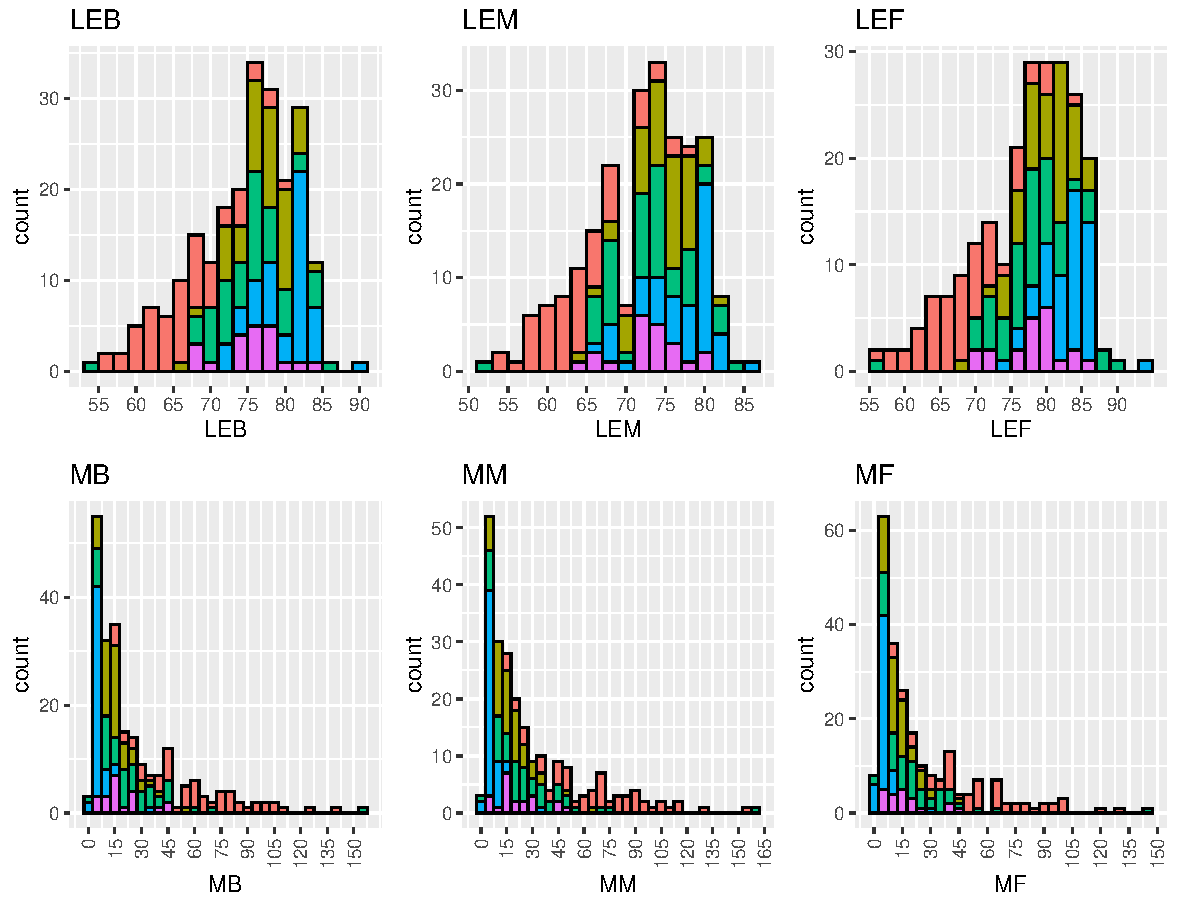
\includegraphics[width=0.7\textwidth]{/Users/user/Desktop/SOSE23/ICS/plot grid of variables.pdf}
\caption{life expectancy and mortality rate of male, female, and  both sexes with the difference in the region.}
\label{fig:histogram}
\end{figure}

\begin{figure}[ht]
\centering
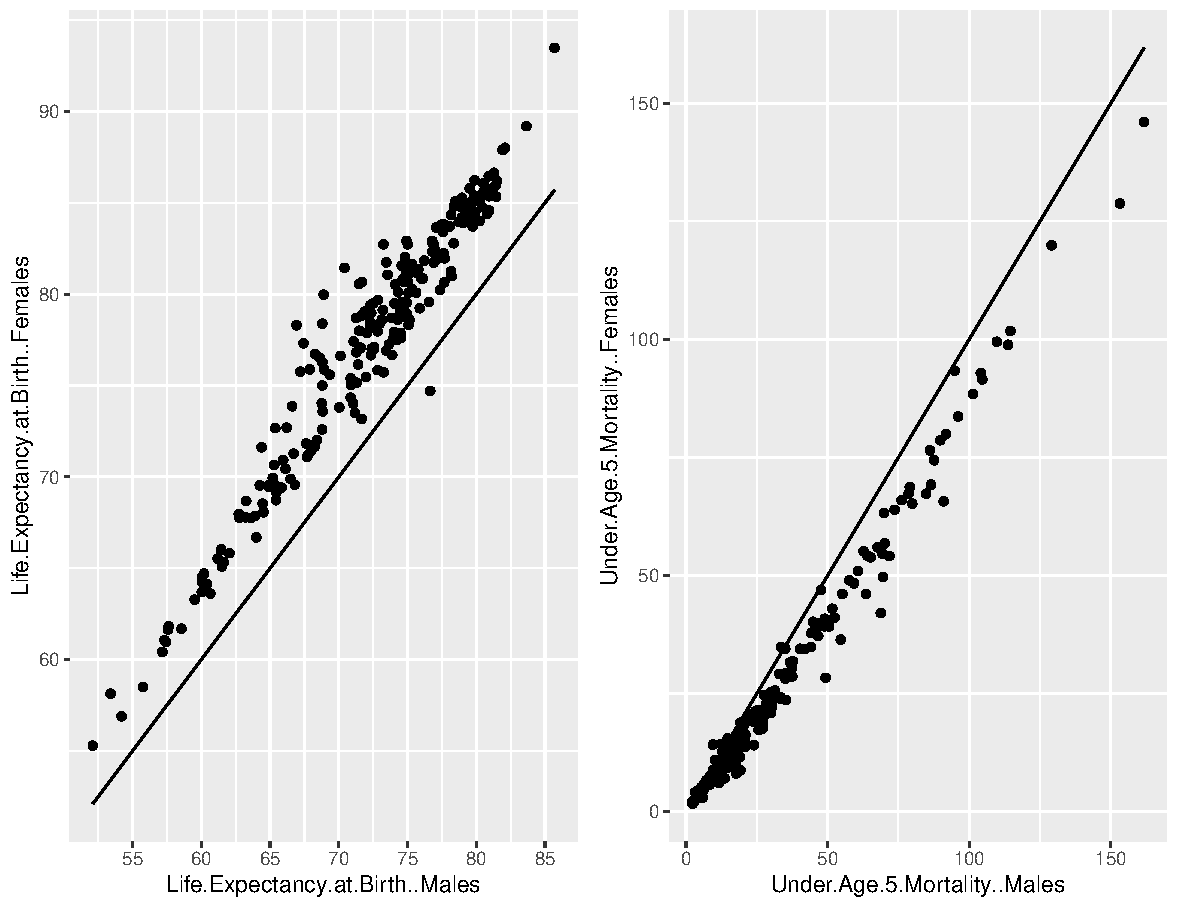
\includegraphics[width=0.7\textwidth]{/Users/user/Desktop/SOSE23/ICS/corelation btw sex of LE and MM.pdf}
\caption{Corelation between sexes of life expectancy at birth and mortality rates.}
\label{fig:histogram}
\end{figure}


\begin{figure}[ht]
\centering
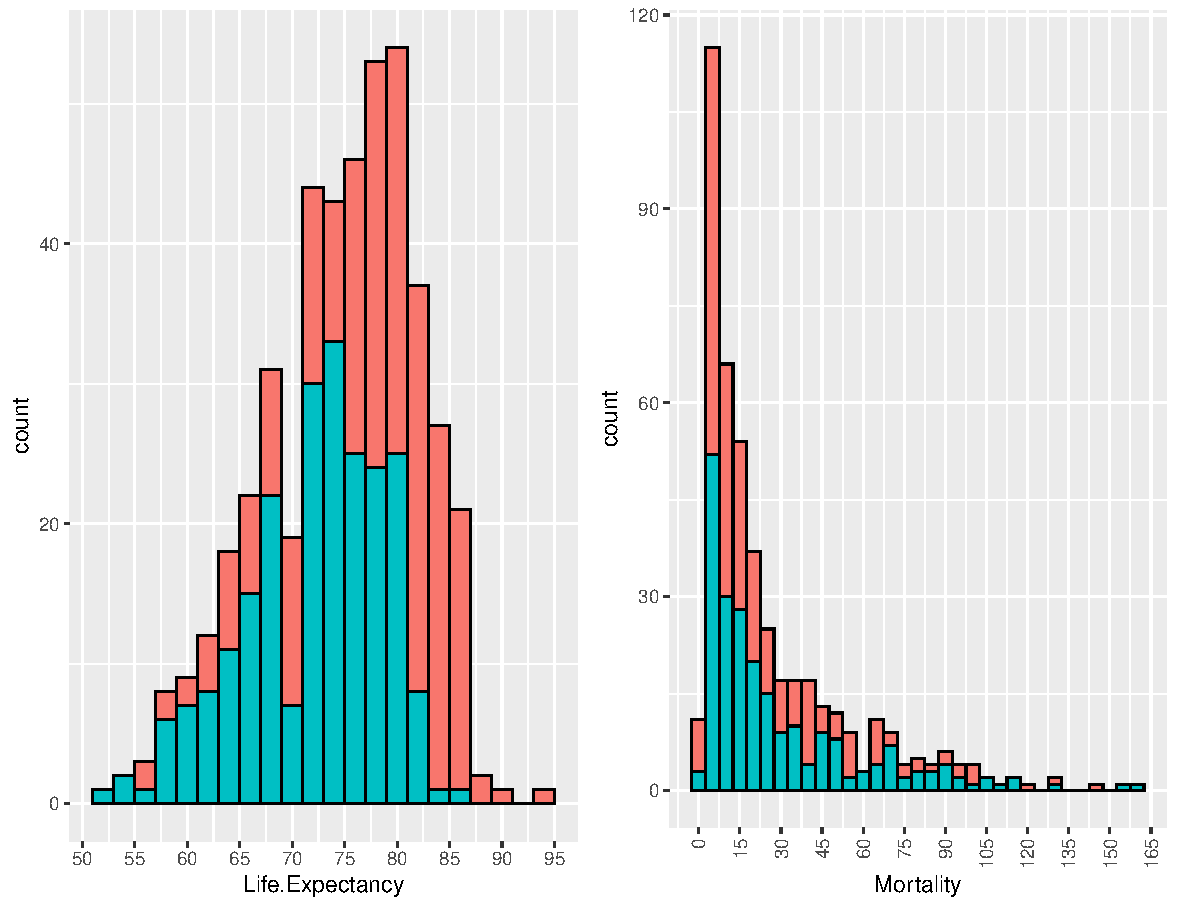
\includegraphics[width=0.7\textwidth]{/Users/user/Desktop/SOSE23/ICS/differences in sex for LE and MR.pdf}
\caption{Differences between sexes of life expectancy at birth and mortality rates.}
\label{fig:histogram}
\end{figure}



In Figure 1, we have a plot grid of histograms showing the frequency distribution of all the nominal variables in our data set. For plots LEB, LEM, and LEF from the shape of the histogram, we observe that the frequency distribution is negatively skewed i.e skewed to the left which means most of the observations in the data set are concentrated on the right side of the distribution and there is a pull the mean and median to the left i.e the mean is less than the median of the distribution. from the histogram of LEB, it can be observed the mean is around 74 while the median is around 76, while for LEM, it can be observed that the mean and median are around 72 and 73 respectively, and for LEF, the mean and median of the distribution around 77 and 78 respectively. We can also observe from bins of plots LEB, LEM, and LEF that the values in these observations are fairly spread over a wide range, and there is a fairly large variation in the data points of the observations i.e. means the data points are less concentrated around the center.

For plots MB, MM, and MF in Figure 1, it can be observed from the shape of the histogram that the frequency distribution is positively skewed i.e skewed to the right, which means the majority of the values in the observations are relatively close to the lower bound values and some rare high values are pushing the mean and median towards the right,i.e the mean is greater than the median of the distributions. From the histogram, it can be observed the mean and median of plots MB, MM, and MF are around 27 and 15, 29 and 17, and 24 and 13 respectively. The bins of the histogram are narrow which indicates less variation in the values for the observations MB, MM, and MF i.e. they are concentrated around the mean of the distribution, and values are less spread out. Also, some values in the observations are slightly different from other values in the observations.

In Figure 1, the difference between the different life expectancies and mortality rates in each region can be seen with the different color codes where and with Africa has the lowest life expectancy and highest mortality rate for both sexes, male and female, while Europe has the highest life expectancy from our data set and Europe has the lowest mortality rate.

In Figure 2, we can see observe from our scatterplot the relationship between sexes of life expectancy and mortality. There is a positive correlation between life expectancy and mortality rates of both males and females which indicates as life expectancy in males increases, life expectancy in females increases also which goes for the same for mortality rates in males and females, as one increases the other increases also.

In Figure 3, from the histogram of life expectancy and mortality, we can deduce that females have higher life expectancy compared to males in our data set and females have a lower mortality rate compared to males.

\subsection{Homogeneity within subregions and heterogeneity between subregions }
 For this task, a boxplot is very appropriate to check the variability of the data set as it provides a graphical representation of the dispersion of data which we would use to check for homogeneity within individual sub-regions and heterogeneity between different sub-regions.
 
 In Figure 4, We picked Asia as our region for the descriptive analysis to check for homogeneity within its subregions and heterogeneity between subregions.
 
 For LEB, LEM, and LEF South Central Asia(SCA) and South Eastern Asia (SEA) are less heterogeneous between subregions as we can deduce because their medians are similar while  Eastern Asia( EA) and Western Asia(WA) are more heterogenous between subregions since their medians are far apart. For homogeneity within subregions, SCA and WA are more homogeneous because they have a smaller interquartile range compared to SEA and EA that has a larger interquartile range and are less homogenous within the subregion
 
For MB, MM, and MF, SEA and WA are less heterogeneous between subregions as we can deduce because their medians are similar while  EA and SCA are more heterogenous between subregions since their medians are far apart. For homogeneity within subregions WA and EA are more homogeneous because they have a smaller interquartile range compared to SCA and SEA that has a larger interquartile range which makes them less homogenous within subregions

\begin{figure}[ht]
\centering
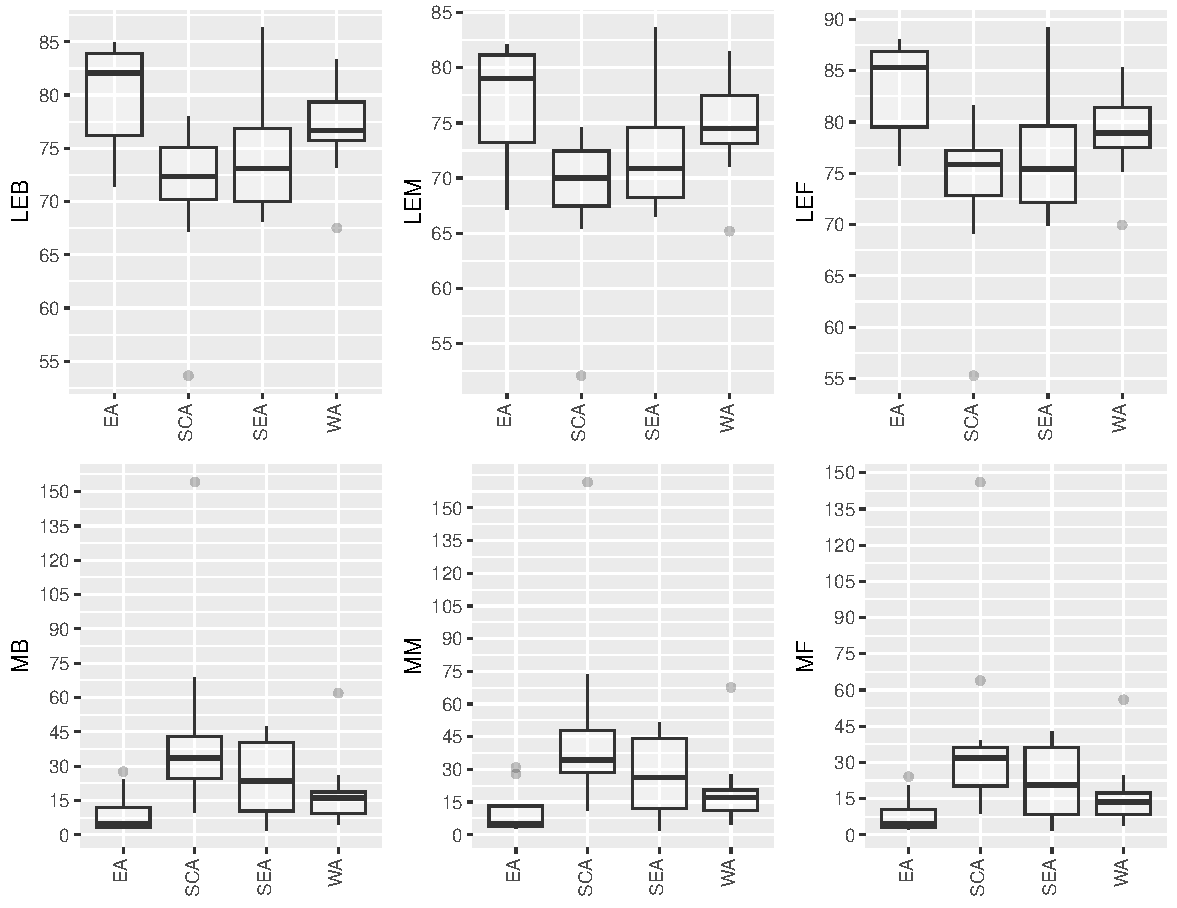
\includegraphics[width=0.7\textwidth]{/Users/user/Desktop/SOSE23/ICS/comparing variability.pdf}
\caption{variablity.}
\label{fig:boxplot}
\end{figure}

 
 
 
 
\subsection{Bivariate correlations between the variables }

From Figure 6,7,8, we can deduce that there is a negative correlation between the variables which means as life expectancy increases in both sexes the mortality rate decreases for both sexes in Figure 6. The same thing goes for Figure 7, as life expectancy in male increase, the mortality rate in male decreases and lastly in figure 8,  as life expectancy increases, the mortality rate decreases.

\begin{table}[ht]
\centering
\captionabove{Correlation coefficient for all pairs of variables}
\label{tab:cor}
\begin{tabular}{l|rrrrrr}
& LEB     & LEM     & LEF     & MB      & MM      & MF      \\
\hline

LEB & 1.0000  & 0.9926  & 0.9929  & -0.8989 & -0.8976 & -0.8970 \\
LEM & 0.9926  & 1.0000  & 0.9712  & -0.8789 & -0.8794 & -0.8749 \\
LEF & 0.9929  & 0.9712  & 1.0000  & -0.9059 & -0.9029 & -0.9060 \\
MB  & -0.8989 & -0.8789 & -0.9059 & 1.0000  & 0.9985  & 0.9979  \\
MM  & -0.8976 & -0.8794 & -0.9029 & 0.9985  & 1.0000  & 0.9929  \\
MF  & -0.8970 & -0.8749 & -0.9060 & 0.9979  & 0.9929  & 1.0000 
\end{tabular}
\end{table}

\begin{figure}[ht]
\centering
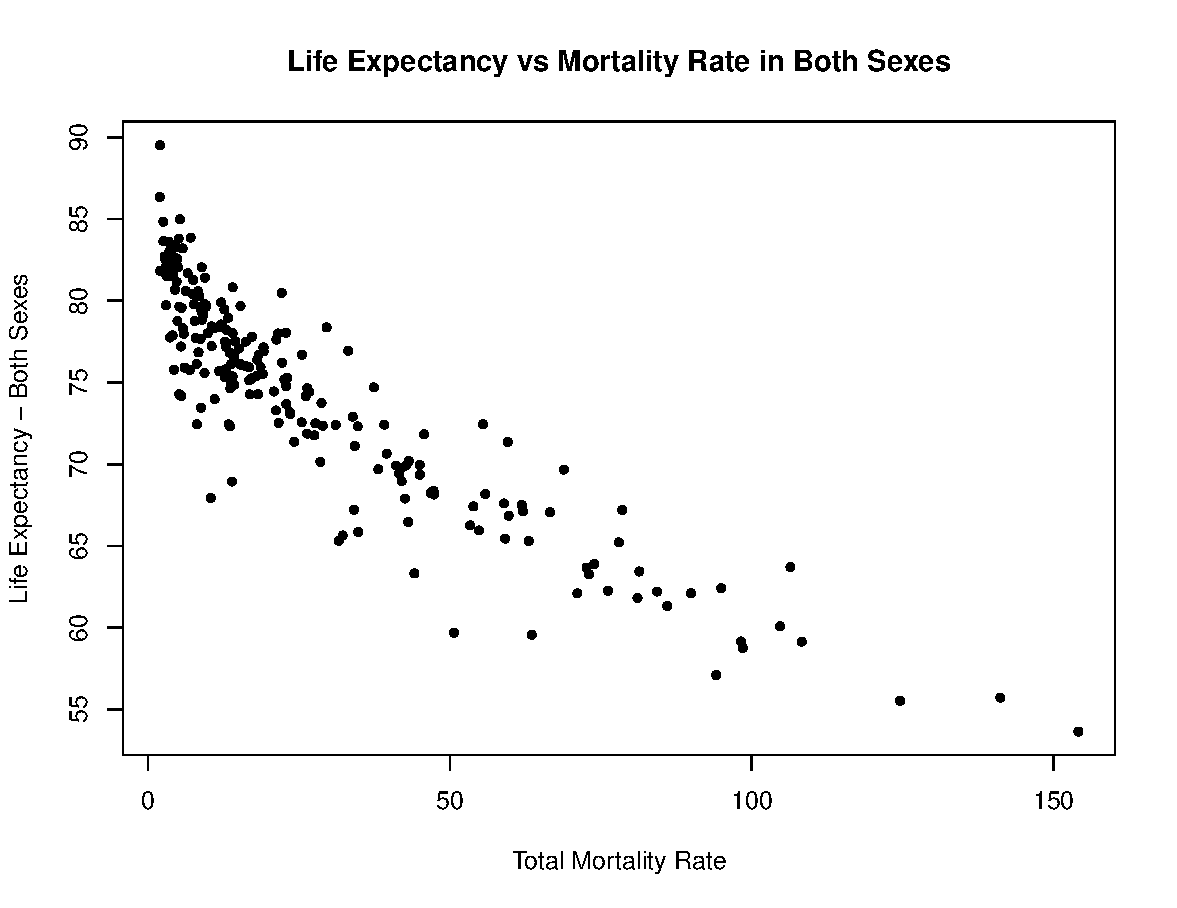
\includegraphics[width=0.7\textwidth]{/Users/user/Desktop/SOSE23/ICS/LE vs MR both sexes.pdf}
\caption{correlation between life expectancy and mortality rate of both sexes.}
\label{fig:scatterplot}
\end{figure}

\begin{figure}[ht]
\centering
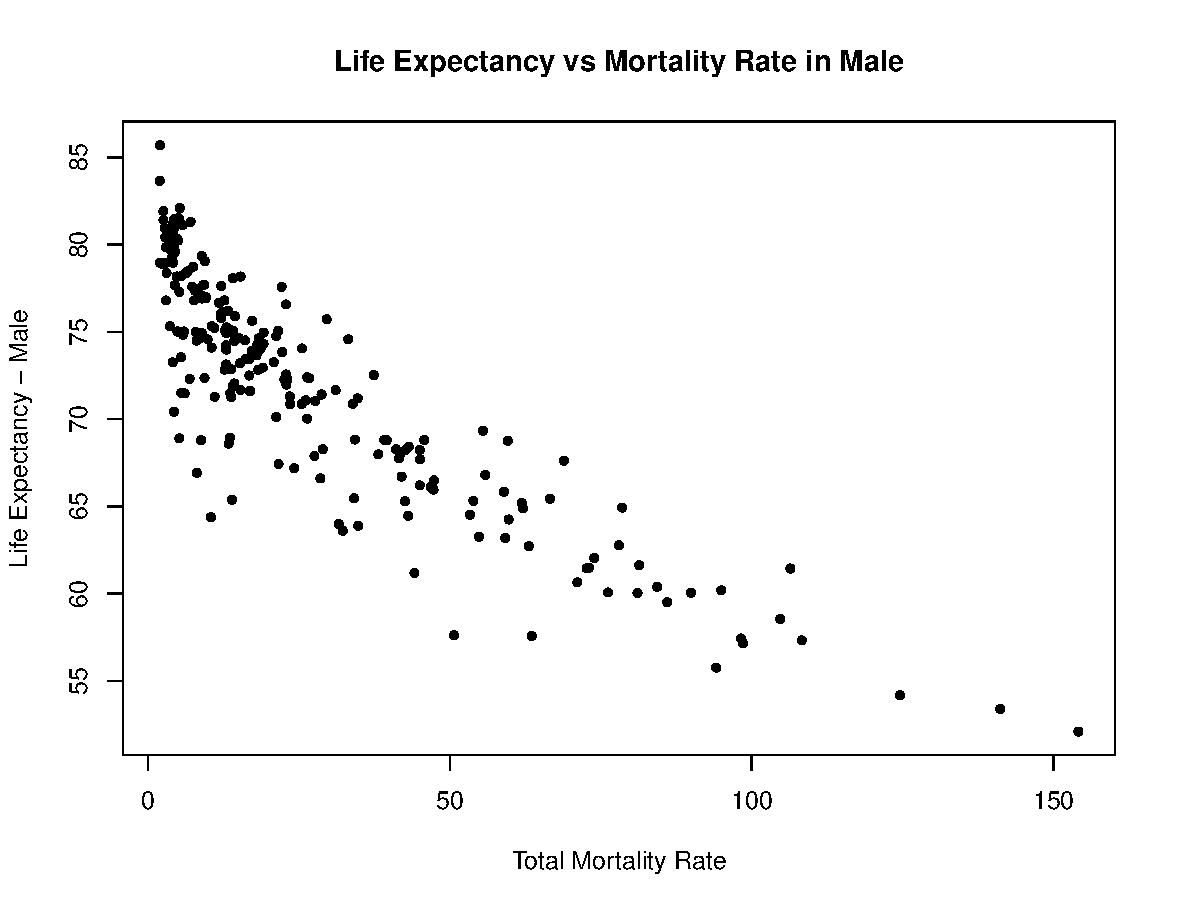
\includegraphics[width=0.7\textwidth]{/Users/user/Desktop/SOSE23/ICS/LE vs MR male task 3.pdf}
\caption{correlation between life expectancy and mortality rate of male}
\label{fig:scatterplot}
\end{figure}

\begin{figure}[ht]
\centering
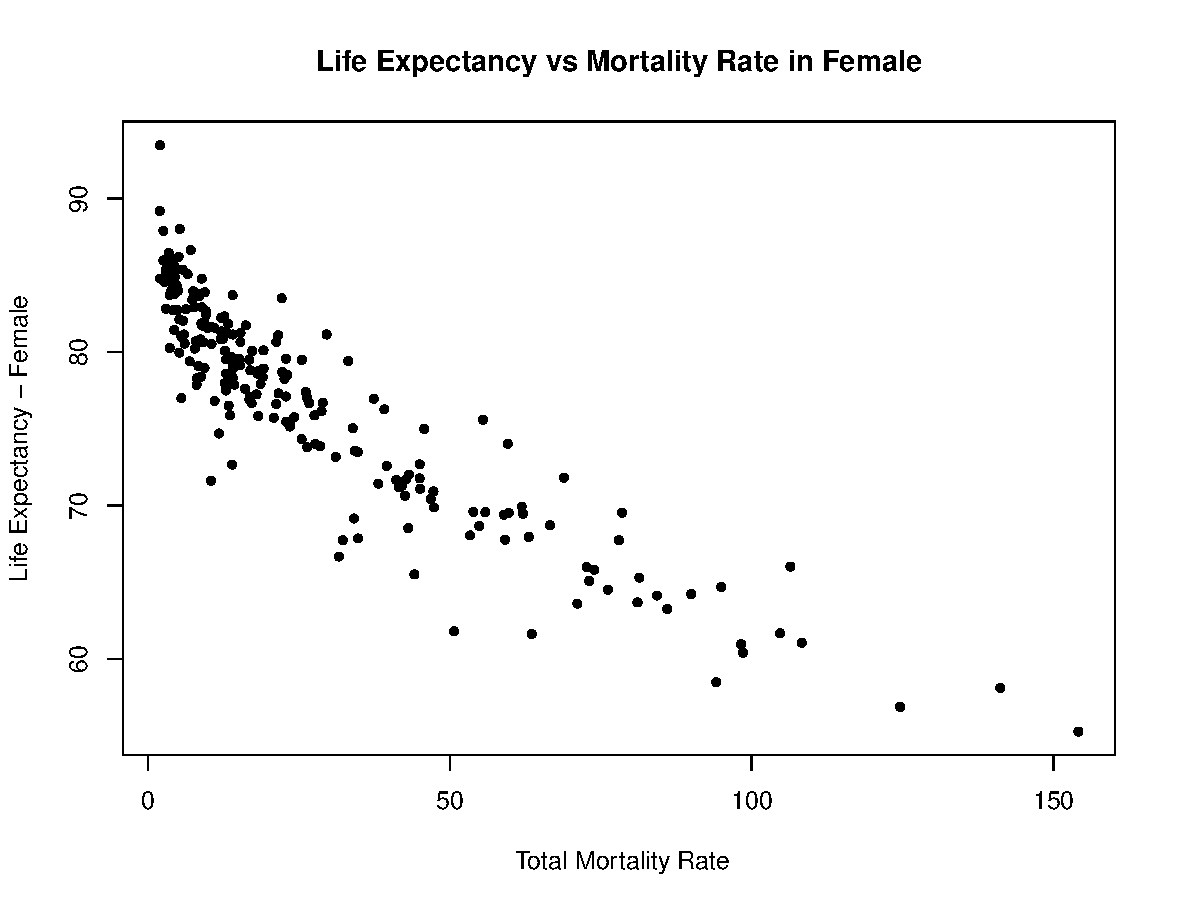
\includegraphics[width=0.7\textwidth]{/Users/user/Desktop/SOSE23/ICS/LE vs MR female.pdf}
\caption{correlation between life expectancy and mortality rate of female}
\label{fig:scatterplot}
\end{figure}


\subsection{Change in variable values over 20 years }
In Figure 8, the change in life expectancy rate over the last 20 for LEB, LEM, and LEF increased because the median is higher in the year 2020 compared to the median of the boxplot in the year 2002 while the change in the mortality rate for MB, MM, MF decreased in the year 2020 compared to the year 2002 as the median reduced over the years.

\begin{figure}[tb]
\centering
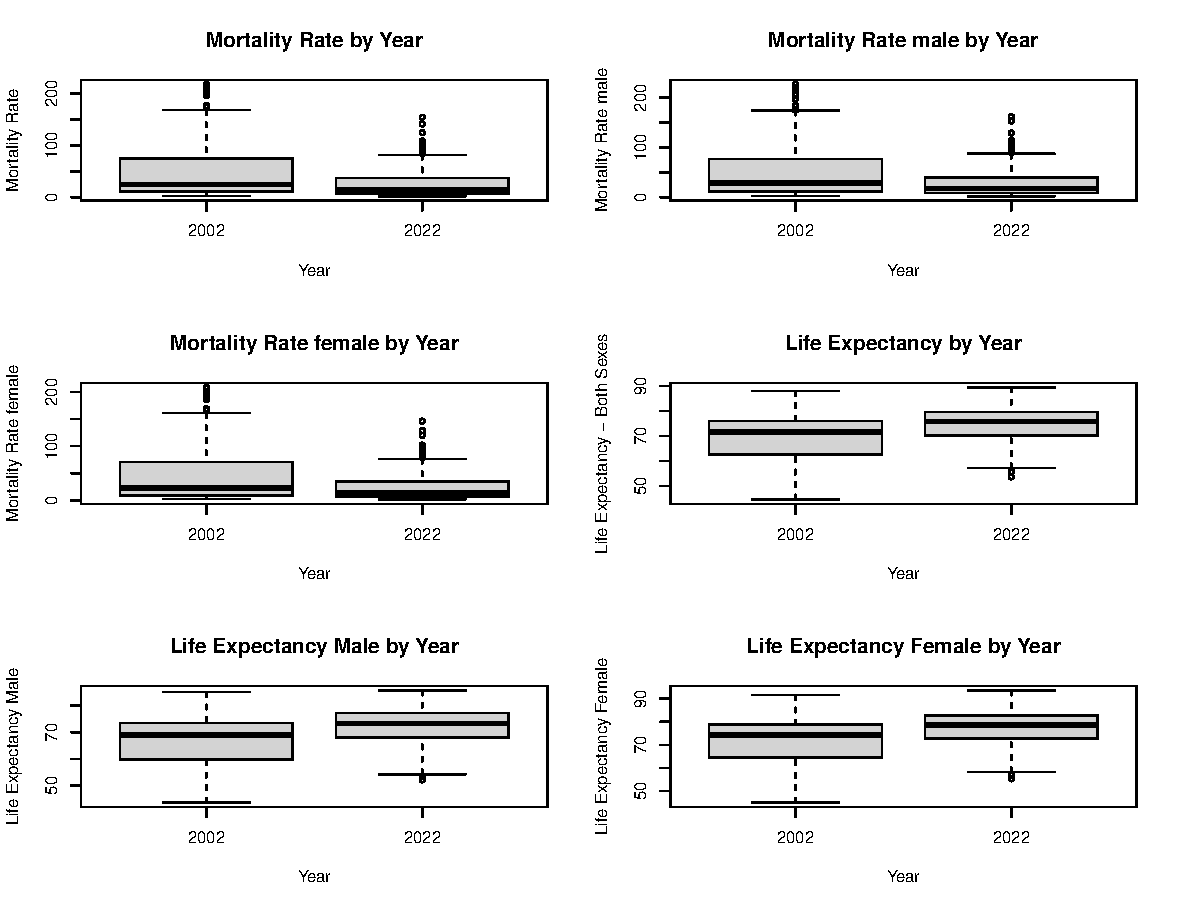
\includegraphics[width=0.7\textwidth]{/Users/user/Desktop/SOSE23/ICS/Change over the years.pdf}
\caption{change in variable values over 20 years}
\label{fig:scatterplot}
\end{figure}







\section{Summary}

The demographic data used for this analysis is a 20-year data set extracted from the international database (IDB) of the U.S Census Bureau on all states and regions that are recognized by the US Department of State and we have been able to describe the frequency distributions of the variables while considering the difference between the sexes and region. Also, we were able to check for homogeneity within subregions and heterogeneity between different subregions using Asia as our example in the analysis. We investigated the relationship between the variables in our dataset to get a deeper understanding of how each variable relates to the other and lastly, analyzed for change in trends over the last 20 years of observation in our dataset.

We found from our analysis that the LEB, LEM, and LEF have a negatively skewed frequency distribution which made the mean less than the median of the distribution of variables with relatively low values in the data set while MB, MM, and MF have a positively skewed frequency distribution which made the mean more than the median in the distribution of variables with some high values in the data set. In plots LEF and LEB, there are some values in both observations that are slightly different from other values in the observations which could have been caused either by errors in data generation or rare events in the observation.
Also, we were able to discover using the subregions in Asia as our example in this report that LEB, LEM, and LEF were less heterogenous between subregions for SCA and SEA while it was more heterogenous in its distribution for EA and WA. And it was more homogeneous within the subregion for SCA and WA while SEA and EA were less homogenous within the subregion. For MB, MM, and MF, the heterogeneity between the sub-regions was less in SEA and WA compared to EA and SCA which had more heterogeneity between the sub-regions, while WA and EA are more homogenous with the subregion than SCA and SEA less homogenous.
The correlation between variables in our data set is negative and finally, the change in life expectancy rate over the years increased while mortality rate decreased. 




\newpage
\addcontentsline{toc}{section}{Bibliography}
\renewcommand\refname{Bibliography} 
\bibliography{references}
\bibliographystyle{apalike}


\newpage
\appendix 
\addsec{Appendix}
\subsection*{A \ Additional figures}
\addcontentsline{toc}{subsection}{A \hspace*{0.15cm} Additional figures} 
\subsection*{B \ Additional tables}
\addcontentsline{toc}{subsection}{B \hspace*{0.15cm} Additional tables} 

\end{document}